\begin{enumerate}
    \item \textbf{Bất đẳng thức Bell.} \\
    \begin{enumerate}[label=\textbf{\alph*,}]\itemsep0em
        \item Do $A(\Vec{a},\lambda)$ và $B(\Vec{b},\lambda)$ là kết quả đo spin của hạt 1 và hạt 2 lần lượt trên vector đơn vị $\Vec{a}$ và $\Vec{b}$ mà $A$ không ảnh hưởng đến $B$ nên $A(\Vec{a},\lambda)$ và $B(\Vec{b},\lambda)$ chỉ nhận giá trị sau:
\begin{align}
    \label{eq1_Bell}
    A(\Vec{a},\lambda)=\Vec{\sigma}_1\cdot \Vec{a}= \pm 1, \\
    \label{eq2_Bell}
    B(\Vec{b},\lambda)=\Vec{\sigma}_2\cdot \Vec{b}= \pm 1.
\end{align}
    \item \begin{enumerate}
        \item Trong trường hợp $\Vec{a}=\Vec{b}$, hai hạt chắc chắn có spin phản song song nhau, khi đó: 
\begin{align}
    \label{eq3_Bell}
    A(\Vec{a},\lambda)=-B(\Vec{a},\lambda),\\
    \label{eq4_Bell}
    A(\Vec{b},\lambda)=-B(\Vec{b},\lambda).
\end{align}
       \item Thay phương trình (\ref{eq1_Bell}) và phương trình (\ref{eq3_Bell}) vào công thức tính giá trị trung bình trong đề bài, ta được giá trị trung bình của kết quả phép đo $\Vec{\sigma}_1$ đo trên $\Vec{a}$ và $\Vec{\sigma}_2$ đo trên $\Vec{b}$ xảy ra đồng thời:
       \begin{align}
    P(\Vec{a},\Vec{a})&=-\displaystyle\int\limits_{-\infty}^{+\infty}A(\Vec{a},\lambda)A(\Vec{a},\lambda)\rho(\lambda)d\lambda=-\displaystyle\int\limits_{-\infty}^{+\infty}\left[A(\Vec{a},\lambda)\right]^2\rho(\lambda)d\lambda \nonumber \\
    \label{eq5_Bell}
    &=-\displaystyle\int\limits_{-\infty}^{+\infty}\rho(\lambda)d\lambda=-1.
\end{align}
        \item Từ kết quả (\ref{eq4_Bell}), thay vào công thức tính giá trị trung bình $P(\Vec{a},\Vec{b})$, ta được:
\begin{align} \label{eq6_Bell}
    P(\Vec{a},\Vec{b})=-\displaystyle\int\limits_{-\infty}^{+\infty}A(\Vec{a},\lambda)A(\Vec{b},\lambda)\rho(\lambda)d\lambda.
\end{align}
    \end{enumerate}
    \item Tương tự kết quả (\ref{eq6_Bell}), ta tổng quát hoá với trường hợp $\Vec{a}$ và $\Vec{c}$, $\Vec{c}$ có vai trò như $\Vec{b}$ nên ta chỉ cần thay $\Vec{b}$ thành $\Vec{c}$:
\begin{align} \label{eq7_Bell}
    P(\Vec{a},\Vec{c})=-\displaystyle\int\limits_{-\infty}^{+\infty}A(\Vec{a},\lambda)A(\Vec{c},\lambda)\rho(\lambda)d\lambda.
\end{align}
    \item \begin{enumerate}
        \item Ta tính hiệu $P(\Vec{a},\Vec{b})-P(\Vec{a},\Vec{c})$ từ phương trình (\ref{eq6_Bell}) và phương trình (\ref{eq7_Bell}):
\begin{align}
    P(\Vec{a},\Vec{b})-P(\Vec{a},\Vec{c})&=-\displaystyle\int\limits_{-\infty}^{+\infty}\left[A(\Vec{a},\lambda)A(\Vec{b},\lambda)-A(\Vec{a},\lambda)A(\Vec{c},\lambda)\right]\rho(\lambda)d\lambda\nonumber \\
    \label{eq8_Bell}
    &=-\displaystyle\int\limits_{-\infty}^{+\infty}\left[1-\dfrac{A(\Vec{c},\lambda)}{A(\Vec{b},\lambda)}\right]A(\Vec{a},\lambda)A(\Vec{b},\lambda)\rho(\lambda)d\lambda.
\end{align}
Vì ta đang cần xuất hiện thành phần $A(\Vec{b},\lambda)A(\Vec{c},\lambda)$ để tạo ra thành phần $P(\Vec{b},\Vec{c})$ nên ta nhân vào trước $A(\Vec{c},\lambda)$ số hạng $\left[A(\Vec{b},\lambda)\right]^2$. Theo kết quả (\ref{eq2_Bell}): $\left[A(\Vec{b},\lambda)\right]^2=1$.
\begin{align}
    P(\Vec{a},\Vec{b})-P(\Vec{a},\Vec{c})&=-\displaystyle\int\limits_{-\infty}^{+\infty}\left[1-\left[A(\Vec{b},\lambda)\right]^2\dfrac{A(\Vec{c},\lambda)}{A(\Vec{b},\lambda)}\right]A(\Vec{a},\lambda)A(\Vec{b},\lambda)\rho(\lambda)d\lambda \nonumber \\
    \label{eq9_Bell}
    &=-\displaystyle\int\limits_{-\infty}^{+\infty}A(\Vec{a},\lambda)A(\Vec{b},\lambda)\left[1-A(\Vec{b},\lambda)A(\Vec{c},\lambda)\right]\rho(\lambda)d\lambda.
\end{align}
Ta nhận xét từ phương trình (\ref{eq9_Bell}): Do các giá trị $A$ chỉ có thể nhận các giá trị $+1$ và $-1$ nên ta có:
\begin{align}
    \label{eq10_Bell}
    -1 \leq A(\Vec{a},\lambda)A(\Vec{b},\lambda) \leq + 1, \\
    \label{eq11_Bell}
    -1 \leq A(\Vec{b},\lambda)A(\Vec{c},\lambda) \leq + 1.
\end{align}
Từ kết quả (\ref{eq11_Bell}), ta nhận thấy: $\left[1-A(\Vec{b},\lambda)A(\Vec{c},\lambda)\right]\rho(\lambda) \geq 0$. \\
\begin{enumerate}
\item Xét trường hợp 1: $0 \leq A(\Vec{a},\lambda)A(\Vec{b},\lambda) \leq + 1$. Rõ ràng ta thấy được:
\begin{align}
    \label{eq12_Bell}
    \hspace{-2cm} 0\geq -\displaystyle\int\limits_{-\infty}^{+\infty}A(\Vec{a},\lambda)A(\Vec{b},\lambda)&\left[ 1-A(\Vec{b},\lambda)A(\Vec{c},\lambda)\right]\rho(\lambda)d\lambda \geq -\displaystyle\int\limits_{-\infty}^{+\infty}\left[1-A(\Vec{b},\lambda)A(\Vec{c},\lambda)\right]\rho(\lambda)d\lambda, \\
    \label{eq13_Bell}
    0& \geq P(\Vec{a},\Vec{b})-P(\Vec{a},\Vec{c}) \geq - 1 - P(\Vec{b},\Vec{c}).
\end{align}
\item Xét trường hợp 2: $-1 \leq A(\Vec{a},\lambda)A(\Vec{b},\lambda) \leq 0$. Rõ ràng ta thấy được:
\begin{align}
    \label{eq14_Bell}
    \hspace{-2cm} 0\leq -\displaystyle\int\limits_{-\infty}^{+\infty}A(\Vec{a},\lambda)A(\Vec{b},\lambda)&\left[ 1-A(\Vec{b},\lambda)A(\Vec{c},\lambda)\right]\rho(\lambda)d\lambda \leq -\displaystyle\int\limits_{-\infty}^{+\infty}\left[1-A(\Vec{b},\lambda)A(\Vec{c},\lambda)\right]\rho(\lambda)d\lambda, \\
    \label{eq15_Bell}
    0& \leq P(\Vec{a},\Vec{b})-P(\Vec{a},\Vec{c}) \leq  1 + P(\Vec{b},\Vec{c}).
\end{align}
\end{enumerate}
Như vậy điều kiện liên hệ giữa $P(\Vec{a},\Vec{b})$, $P(\Vec{a},\Vec{c})$ và $P(\Vec{b},\Vec{c})$ từ bất đẳng thức (\ref{eq13_Bell}) và (\ref{eq15_Bell}) là:
\begin{align} \label{eq16_Bell}
    \begin{cases}
    0\leq \ P(\Vec{a},\Vec{c})-P(\Vec{a},\Vec{b})&\leq  1 + P(\Vec{b},\Vec{c}),\\
    0\leq \ P(\Vec{a},\Vec{b})-P(\Vec{a},\Vec{c})&\leq  1 + P(\Vec{b},\Vec{c}).
    \end{cases}
\end{align}
Bất đẳng thức (\ref{eq16_Bell}) có thể viết lại thành:
\begin{align} \label{eq17_Bell}
    \big|P(\Vec{a},\Vec{b})-P(\Vec{a},\Vec{c})\big|&\leq  1 + P(\Vec{b},\Vec{c}).
\end{align}
      \item Thay số theo đề bài:
\begin{align}
    \label{eq18_Bell}
    P(\Vec{a},\Vec{b})&=-\Vec{a}\cdot \Vec{b}=0,\\
    \label{eq19_Bell}
    P(\Vec{a},\Vec{c})&=-\Vec{a}\cdot \Vec{c}=-\dfrac{1}{\sqrt{2}},\\
    \label{eq20_Bell}
    P(\Vec{b},\Vec{c})&=-\Vec{b}\cdot \Vec{c}=-\dfrac{1}{\sqrt{2}}.
\end{align}
Như vậy, từ (\ref{eq17_Bell}), (\ref{eq18_Bell}), (\ref{eq19_Bell}) và (\ref{eq20_Bell}), rõ ràng điều kiện (\ref{eq17_Bell}) bị vi phạm vì: 
$$\left|0+\dfrac{1}{\sqrt{2}}\right| \leq 1-\dfrac{1}{\sqrt{2}}.$$
Kết quả này là vô lý và trường hợp cụ thể này không tồn tại. Vì ta đã xây dựng bài toán và điều kiện (\ref{eq17_Bell}) theo lý thuyết biến ẩn nên trường hợp bị vi phạm đã chỉ ra không tồn tại lý thuyết biến ẩn và cơ học lượng tử theo quan điểm của Bohr đúng.
    \end{enumerate}
    \end{enumerate}
\textit{Bất đẳng thức (\ref{eq17_Bell}) chính xác là bất đẳng thức Bell nổi tiếng, công trình này khi ra đời đã giúp loại bỏ lý thuyết biến số ẩn khỏi cơ học lượng tử và kết luận rằng việc thực hiện phép đo ở một vị trí trong không gian này có thể ảnh hưởng tức thì đến phép đo ở vị trí khác trong không gian kia. Sự ảnh hưởng này là tức thời bất kể khoảng cách, Bell đã thừa nhận sự tồn tại của "tác dụng ma quái theo khoảng cách". Tuy nhiên, các nhà khoa học dù phần lớn tin vào trường phái Copenhagen của Bohr nhưng vẫn có những người vẫn chọn tin vào Einstein, đều đó mới dẫn đến các thí nghiệm kiểm chứng bất đẳng thức Bell sau này của Clauser, Aspect và Zeilinger.}

    \item \textbf{Kiểm chứng bất đẳng thức Bell bằng thực nghiệm và giải Nobel 2022.} \\
    \begin{enumerate}[label=\textbf{\alph*,}]\itemsep0em
        \item Khi phương phân cực của hai kính giống nhau $\Vec{a}=\Vec{b}$,     xác suất để hai photon cùng đi qua bằng xác suất để cùng không đi qua và không tồn tại trường hợp chỉ một trong hai đi qua, do:
\begin{align}
    \label{eq21_Bell}
    P_{++}(\Vec{a},\Vec{a})=P_{--}(\Vec{a},\Vec{a})=\dfrac{1}{2},\\
    \label{eq22_Bell}
    P_{+-}(\Vec{a},\Vec{a})=P_{-+}(\Vec{a},\Vec{a})=0.
\end{align}
    \item "Tương quan" giữa hai photon theo diễn giải của Bohr:
\begin{align}
    E(\Vec{a},\Vec{b})&=P_{++}(\Vec{a},\Vec{b})+P_{--}(\Vec{a},\Vec{b})-P_{+-}(\Vec{a},\Vec{b})-P_{-+}(\Vec{a},\Vec{b})\nonumber \\
    \label{eq23_Bell}
    &=\cos^2\theta - \sin^2\theta = \cos 2 \theta.
\end{align} 
     \item \begin{enumerate}
         \item Ta biến đổi đại lượng $s(\Vec{a},\Vec{a'},\Vec{b},\Vec{b'},\lambda)$:
\begin{align}
    s(\Vec{a},\Vec{a'},\Vec{b},\Vec{b'},\lambda)&=A(\Vec{a},\lambda)B(\Vec{b},\lambda)-A(\Vec{a},\lambda)B(\Vec{b'},\lambda)+A(\Vec{a'},\lambda)B(\Vec{b},\lambda)+A(\Vec{a'},\lambda)B(\Vec{b'},\lambda) \nonumber \\ 
    \label{eq24_Bell}
    &=A(\Vec{a},\lambda)\left[B(\Vec{b},\lambda)-B(\Vec{b'},\lambda)\right]+A(\Vec{a'},\lambda)\left[B(\Vec{b},\lambda)+B(\Vec{b'},\lambda)\right].
\end{align}
Từ đề bài, do $A$ và $B$ chỉ có thể nhận giá trị $-1$ hoặc $+1$ nên $s(\Vec{a},\Vec{a'},\Vec{b},\Vec{b'},\lambda)$ chỉ có thể nhận giá trị $+2$ hoặc $-2$. 
\item Giả sử lý thuyết biến ẩn tồn tại và diễn giải của Bohr sai. Giá trị trung bình $S(\Vec{a},\Vec{a'},\Vec{b},\Vec{b'})$ của $s(\Vec{a},\Vec{a'},\Vec{b},\Vec{b'},\lambda)$ là phải nằm trong khoảng $-2$ đến $+2$ do $s(\Vec{a},\Vec{a'},\Vec{b},\Vec{b'},\lambda)$ chỉ có thể nhận giá trị $+2$ hoặc $-2$ (giả sử ta đo ra $m$ giá trị $+2$, $n$ giá trị $-2$, trung bình sẽ là $\dfrac{2(m-n)}{m+n}$ và nằm trong khoảng $-2$ đến $+2$)
\begin{align} \label{eq25_Bell}
    -2\leq S(\Vec{a},\Vec{a'},\Vec{b},\Vec{b'}) \leq 2.
\end{align}
Ngoài ra, khi ta sử dụng định nghĩa giá trị trung bình trong đề bài, ta thu được như sau:
\begin{align}
    S(\Vec{a},\Vec{a'},\Vec{b},\Vec{b'})&=\displaystyle\int\limits_{-\infty}^{+\infty}s(\Vec{a},\Vec{a'},\Vec{b},\Vec{b'},\lambda)\rho(\lambda)d\lambda \nonumber \\
    \label{eq26_Bell}
    &=E(\Vec{a},\Vec{b})-E(\Vec{a},\Vec{b'})+E(\Vec{a'},\Vec{b})+E(\Vec{a'},\Vec{b'}).
\end{align}
Đây chính là biểu diễn của đại lượng $S(\Vec{a},\Vec{a'},\Vec{b},\Vec{b'})$.
\item Giả sử lý thuyết biến ẩn không tồn tại và diễn giải của Bohr đúng. Giá trị trung bình $S(\Vec{a},\Vec{a'},\Vec{b},\Vec{b'})$ so với xây dựng từ lý thuyết biến ẩn đều phải mô tả cùng một đại lượng vật lý nào đó. Từ phương trình (\ref{eq23_Bell}) và phương trình (\ref{eq26_Bell}):
\begin{align}
    S(\Vec{a},\Vec{a'},\Vec{b},\Vec{b'})&=E(\Vec{a},\Vec{b})-E(\Vec{a},\Vec{b'})+E(\Vec{a'},\Vec{b})+E(\Vec{a'},\Vec{b'}) \nonumber \\
    &= \cos 2\theta - \cos 6\theta + \cos 2\theta + \cos 2\theta \nonumber \\
    \label{eq27_Bell}
    &= 3\cos 2\theta - \cos 6\theta.
\end{align}
Đại lượng $S(\Vec{a},\Vec{a'},\Vec{b},\Vec{b'})$ đạt cực trị khi $\dfrac{dS}{d\theta}=0$:
\begin{align}
    &\ \ \ \ \ \ \ \ \ \ \ \ \ \ \ \ \ \ \ \ \ \ \ \ \ \ \ \ \ \ \ \ \ \    \dfrac{dS}{d\theta}=0 \nonumber \\
    &\ \ \ \ \ \ \ \ \ \ \ \ \ \ \ \ \ \ \ \ \ \ \ \ \ \ \sin 6\theta - \sin 2\theta =0 \nonumber \\
    &\ \ \  2\sin 2\theta \cos^2 2\theta + \sin 2\theta \left(\cos^2 2\theta - \sin^2 2\theta\right)-\sin 2\theta = 0\nonumber \\
    &\sin 2\theta \left(2 \cos^2 2\theta + \cos^2 2\theta - \sin^2 2\theta -\cos^2 2\theta-\sin^2 2\theta\right)=0\nonumber \\
    \label{eq28_Bell}
    &\ \ \ \ \ \ \ \ \ \ \ \ \ \ \ \ \ \ \ \ \ \ \ \ \ \ \  \sin 2\theta \cos 4\theta =0.
\end{align}
Từ phương trình (\ref{eq28_Bell}), suy ra cực trị của $S(\Vec{a},\Vec{a'},\Vec{b},\Vec{b'})$ \Big(do $S(\theta)$ là hàm lượng giác có công thức như (\ref{eq27_Bell}) nên để tìm cực trị của $S$ ta chỉ cần xét $-\dfrac{\pi}{2}\leq \theta \leq +\dfrac{\pi}{2}$\Big):
\begin{align} \label{eq29_Bell}
    \begin{cases}
        \theta_{\text{extr}} =0,\pm \dfrac{ \pi}{2}\ \ \ \ \ \ \ \ \ \ \ \ S_{\text{extr}} = \pm 2, \\ \\
        \theta_{\text{extr}} = \pm\dfrac{3\pi}{8}\ \ \ \ \ \ \ \ \ \ \ \ \   S_{\text{extr}} =  -2\sqrt{2}, \\ \\
        \theta_{\text{extr}} = \pm\dfrac{\pi}{8}\ \ \ \ \ \ \ \ \ \ \ \ \ \ \  S_{\text{extr}} = +2\sqrt{2}.
    \end{cases}
\end{align}
Như vậy, theo quan điểm cơ học lượng tử của Bohr, điều kiện biên của $S(\Vec{a},\Vec{a'},\Vec{b},\Vec{b'})$:
\begin{align} \label{eq30_Bell}
    -2\sqrt{2}\leq S(\Vec{a},\Vec{a'},\Vec{b},\Vec{b'}) \leq +2\sqrt{2}.
\end{align}
\item Từ bất đẳng thức (\ref{eq25_Bell}) và bất đẳng thức (\ref{eq30_Bell}), nếu tồn tại kết quả thực nghiệm nằm trong khoảng $[-2\sqrt{2},-2]$ và $[2,2\sqrt{2}]$ thì có thể kết luận quan điểm cơ học lượng tử của Bohr đúng.\\
\end{enumerate}
\begin{itemize}
    \item Diễn giải suy sập hàm sóng do phép đo của Bohr: $$-2\sqrt{2}\leq S(\Vec{a},\Vec{a'},\Vec{b},\Vec{b'}) \leq +2\sqrt{2}.$$
    \item Lý thuyết biến số ẩn của Einstein:   $$-2\leq S(\Vec{a},\Vec{a'},\Vec{b},\Vec{b'}) \leq +2.$$
\end{itemize}
\begin{center}
    \begin{figure}[htp]
    \begin{center}
        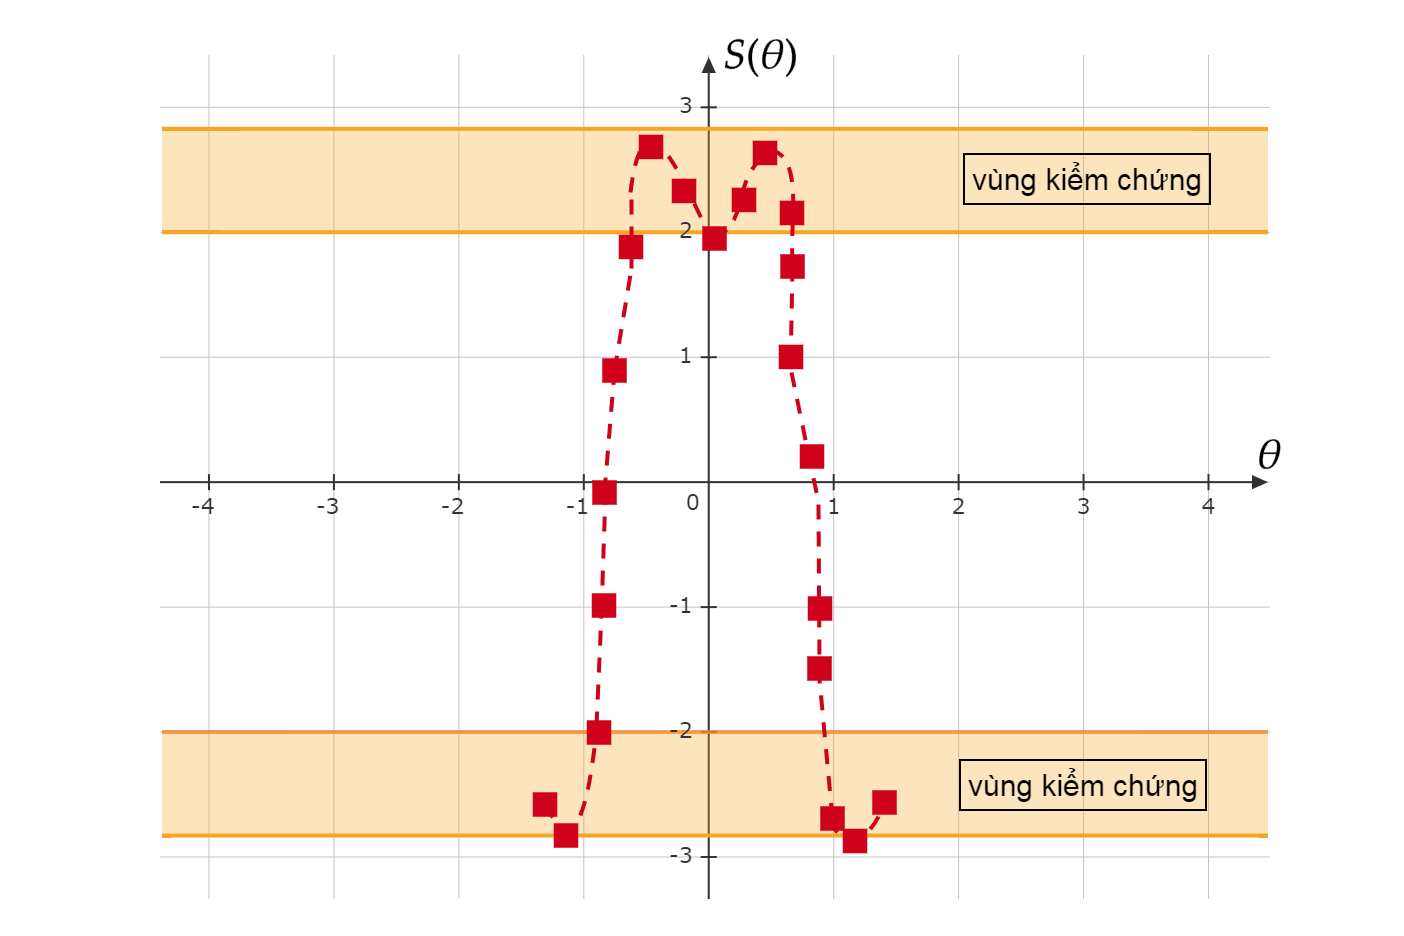
\includegraphics[scale=.22
        ]{Problem_15/image/4.png}
    \end{center}
    \begin{center}
        Hình 4: Tồn tại các kết quả thực nghiệm nằm trong khoản $[-2\sqrt{2},-2]$ và $[2,2\sqrt{2}]$.
    \end{center}
    \end{figure}
\end{center}
Từ đồ thị \textbf{(Hình 4)} ta thấy kết quả thực nghiệm đã chỉ ra diễn giải của Bohr đúng và lý thuyết biến ẩn không tồn tại. Vậy Einstein đã sai và Bohr đã đúng về sự tồn tại của biến số ẩn!
     \end{enumerate}
     \textit{Bất đẳng thức (\ref{eq25_Bell}) là bất đẳng thức CHSH mang chữ cái đầu của 4 tác giả Clauser, Horne, Shimony và Holt. Đây là cách thể hiện khác của bất đẳng thức Bell, được đề xuất bằng cách thay việc đo spin của các hạt thực bằng việc đo hướng phân cực của photon. Kết quả thực nghiệm của các nhà vật lý đã chỉ ra không có biến số ẩn, các hạt vi mô không có định xứ, sự rối lượng tử giữa các hạt là tức thời bất kể khoảng cách bao xa, "tác dụng ma quái theo khoảng cách" không chỉ có thật mà còn là bản chất của các hạt vi mô. Ngoài ra "tác dụng ma quái theo khoảng cách" cũng không còn ma quái khi các nhà khoa học đã chứng minh nó không vi phạm thuyết tương đối vì không có thông tin nào được truyền đi giữa các hạt.}
    \end{enumerate}

\textbf{Biểu điểm}
\begin{center}
\begin{tabular}{|>{\centering\arraybackslash}m{1cm}|>{\raggedright\arraybackslash}m{14cm}| >{\centering\arraybackslash}m{1cm}|}
    \hline
    \textbf{Phần} & \textbf{Nội dung} & \textbf{Điểm} \\
    \hline
    \textbf{1a} & Viết được kết quả (\ref{eq1_Bell}) và (\ref{eq2_Bell}) & $0.50$ \\
    \hline 
    \textbf{1b.i} & Viết được kết quả (\ref{eq3_Bell}) và (\ref{eq4_Bell}) & $0.50$ \\
    \hline 
    \textbf{1b.ii} & Viết được kết quả (\ref{eq5_Bell}) & $0.50$ \\
    \hline 
    \textbf{1b.iii} & Viết được kết quả (\ref{eq6_Bell}) & $0.50$ \\
    \hline 
    \textbf{1c} & Viết được kết quả (\ref{eq7_Bell}) & $0.50$ \\
    \hline 
    \textbf{1d.i} & Viết biểu thức hiệu $P(\Vec{a},\Vec{b})-P(\Vec{a},\Vec{c})$ (\ref{eq9_Bell}) & $2.00$ \\
    \cline{2-3}
    &  Viết được bất đẳng thức (\ref{eq10_Bell}) và (\ref{eq11_Bell}) & $0.50$ \\
    \cline{2-3}
    &  Viết được bất đẳng thức (\ref{eq16_Bell}) hoặc (\ref{eq17_Bell}) & $2.00$ \\
    \hline
    \textbf{1d.ii} & Chỉ ra bất đẳng thức (\ref{eq17_Bell}) bị vi phạm & $0.50$ \\
    \cline{2-3}
    &  Kết luận về sự tồn tại của biến số ẩn & $0.50$ \\
    \hline
    \textbf{2a} & Viết được kết quả (\ref{eq21_Bell}) và (\ref{eq22_Bell}) & $0.50$ \\
    \hline
    \textbf{2b} & Viết biểu thức "tương quan" giữa hai photon theo diễn giải của Bohr (\ref{eq23_Bell}) & $0.50$ \\
    \hline
    \textbf{2c.i} & Viết được biểu thức (\ref{eq24_Bell}) & $0.50$ \\
    \hline
    \textbf{2c.ii} & Chỉ ra đại lượng $s(\Vec{a},\Vec{a'},\Vec{b},\Vec{b'},\lambda)$ chỉ có thể nhận các giá trị $\pm 2$ & $0.50$ \\
    \cline{2-3}
    & Viết được bất đẳng thức (\ref{eq25_Bell}) & $1.50$ \\
    \cline{2-3}
    & Viết được biểu thức (\ref{eq26_Bell}) & $0.50$ \\
    \hline
    \textbf{2c.iii} & Viết được biểu thức (\ref{eq27_Bell}) & $0.50$ \\
    \cline{2-3}
    & Tìm được các cực trị của đại lượng $S$ (\ref{eq29_Bell}) & $1.50$ \\
    \cline{2-3}
    & Viết được bất đẳng thức (\ref{eq30_Bell}) & $1.50$ \\
    \hline
    \textbf{2c.iv} & Lập luận và so sánh với kết quả trong đồ thị. Kết luận. & $0.50$ \\
    \hline
\end{tabular}
\end{center}

%% Reference %%
\bibliographystyle{plain}
\begin{thebibliography}{}
\bibitem{bell1964} John S. Bell (1964), \textit{On the Einstein Podolsky Rosen paradox}, Physics Physique Fizika 1, 195 – Published 1 November 1964.        
\bibitem{clauser1970} John F. Clauser, Michael A. Horne, Abner Shimony, and Richard A. Holt (1970), \textit{Proposed Experiment to Test Local Hidden-Variable Theories}, Physical Review Letters, Volume 23, Issue 15, Pages 880-884.
\bibitem{aspect1976} Alain Aspect (1976), \textit{Proposed experiment to test the nonseparability of quantum mechanics}, Physical Review D, Volume 14, Issue 8, Pages 1944-1951.
\end{thebibliography}

